\graphicspath{{./PBL/images}}

\chapter{Projekt PBL}

Uczenie poprzez realizację projektów (ang. \angver{Project Based Learning}, PBL) jest metodą uczenia 

\section{Cel projektu} \label{cel_projektu}

Celem wspomnianego projektu było zaprojektowanie układu laboratoryjnego, składającego się z klatki Helmholtza oraz umieszczonego wewnątrz klinostatu trójwymiarowego. Docelowo taki układ pozwalałby na przeprowadzanie badań nad rozwojem roślin w warunkach symulowanej mikrograwitacji bez ziemskiego pola magnetycznego. Klatka Helmholtza jest złożeniem trzech par cewek Helmholtza w takiej konfiguracji aby osie magnetyczne każdej z par było prostopadłe do pozostałych. Pozwala to wytworzyć wektor indukjcji magnetycznej o dowolnym kierunku przestrzennym i bardzo wysokiej jednorodności. Wysoka jednorodność jest kluczowa aby generowany wektor indukcji magnetycznej był stały w objętości przeprowadzanego eksperymentu. W związku z wymaganiami projektu, wewnętrzna konstrukcja klinostatu musiała zostać wykonana tak, aby mieć jak najmniejszy wpływ na panujące wewnątrz warunki magnetyczne. Naturalnie rodzi to zagadnienie wyboru materiałów konstrukcyjnych klinostatu, które nie powinny mieć właściwości ferromagnetycznych, powinny mieć względnie niską przewodność elektryczną w celu eliminacji indukowanych prądów wirowych oraz dodatkowym ich atutem będzie niska podatność magnetyczna. Oprócz właściwości magnetycznych materiałów istnotne są też możliwości ich obróbki termicznej oraz mechanicznej, a również ich forma, co później ma wpływ na prostotę montażu urządzenia. Oprócz samych wymagań materiałowych oraz konstrukcyjnych, należało również zapewnić optymalne warunki wzrostowe obiektów badawczych, należało określić odpowiedni rozmiar cewek, aby objętość o wysokim stopniu jednorodności magnetycznej była odpowiednio duża oraz wiele innych. Taki szereg wymagań stworzył bardzo ciekawe i multidyscyplinarne wyzwanie inżynieryjne, które wymagało użycia oraz w niektórych przypadkach stworzenia wielu środowisk symulacyjnych w celu jego rozwiązania. Projekt wykonywany był w zespole 5-cio osobowym na przestrzeni jednego semestru. Powstały na rzecz projektu model komputerowy układu klinostatu wraz z klatką Helmholtza przedstawiony został na Rys. \ref{fig:klatka_helmholtza}.

\begin{figure}
	\centering
	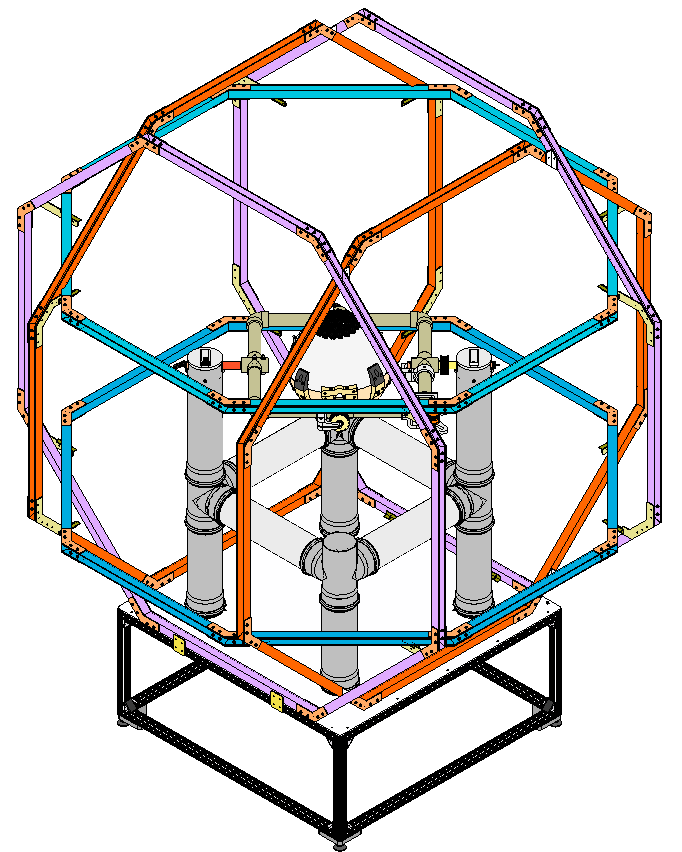
\includegraphics[scale=0.5]{klinostat_klatka}
	\caption{Projekt klatki Helmholtza z klinostatem.} 
	\caption*{Źródło: opracowanie własne}
	\label{fig:klatka_helmholtza}
\end{figure}

\section{Konstrukcja klinostatu}

Ten podrozdział poświęcony został krótkiemu opisowi konstrukcji samego klinostatu zaprojektowanego w ramach PBL. Zaprojektowane urządzenie jest klinostatem o dwóch stopniach swobody, każdy stopień posiada swój osobny napęd. Oznacza to iż jest to maszyna RPM, natomiast jest możliwość uruchomienia go w trybach klinostatu 2-D oraz 3-D jak opisano w podrozdziale \ref{klinostat3d}. Zewnętrzna rama klinostatu wykonana została z rur polipropylenowych (PP) stabilizowanych włóknem szklanym. Odcinki rur wraz z kształtkami 90$^\circ$ oraz czwórnikami zostały połączone metodą polifuzji termicznej (zgrzewanie). Tego typu rury wykorzystywane są w instalacjach centralnego ogrzewania, dzięki czemu ich koszt jest niski. Konstrukcję ramy przedstawiono na Rys. \ref{fig:rama_klinostatu}. Przeprowadzone analizy elementów skończonych (FEM), wskazały iż materiał ten posiada wystarczającą wytrzymałość aby wykorzystać go jako element strukturalny ramy klinostatu. Jako wał obrotowy wykorzystano rurę aluminiową o średnicy \SI{12}{mm}. Wykorzystanie konwencjonalnych łożysk kulowych w konstrukcji klinostatu nie było wskazane ze względu na wymagania opisane w podrozdziale \ref{cel_projektu}. Z tego powodu każdy z interfejsów obrotowych stanowią tuleje ślizgowe wykonane z materiału iglidur$\copyright$, zaprojektowanego przez firmę IGUS. Większość pozostałych elementów została wykonana w technologii druku przestrzennego z materiału PETG. Konstrukcję jednego z czterech czwórników ramy przedstawiono na Rys. \ref{fig:czwórnik}. Wewnętrzny stopień swobody składa się z kulistej komory środowiskowej, która posiada swój dedykowany komputer o niskiej mocy, monitorujący panujące wewnątrz warunki, oraz sterujący oświetleniem. Zasilanie do wnętrza komory doprowadzone jest przez szereg złącz ślizgowych, a przewody poprowadzone są wewnątrz ramy klinostatu. Podobne rozwiązanie wykorzystano w obwodzie doprowadzjącym wodę, przewody prowadzone są wewnątrz ramy klinostatu, a przy elementach obrotowych zastosowano kolanka obrotowe. Rozmiar komory oraz typ i moc oświetlenia zostały wyznaczone na podstawie wyników symulacji stworzonych na rzecz projektu. Jej projekt przedstawiony został na Rys. \ref{fig:komora}. Mocowania śrubowe zostały w większości zrealizowane za pomocą śrub poliamidowych (PA). Komora została zaprojektowana tak, aby umożliwić operatorowi dostęp do jej wnętrza bez konieczności jej demontażu z ramy klinostatu.

\begin{figure}
	\centering
	
	\begin{subfigure}[b]{.49\textwidth}
		\centering
		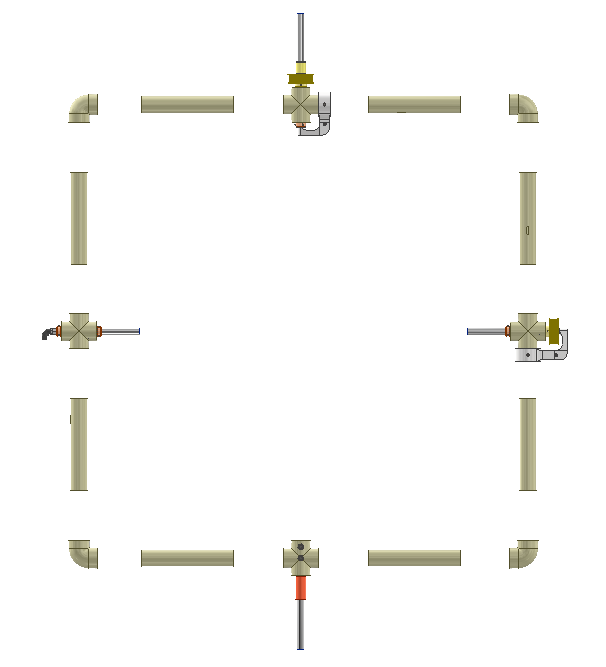
\includegraphics[width=\textwidth]{rama_40_aisass}
		\caption{Rama klinostatu} 
		\label{fig:rama_klinostatu}
	\end{subfigure}
	\hfill%
	\begin{subfigure}[b]{.49\textwidth}
		\centering
		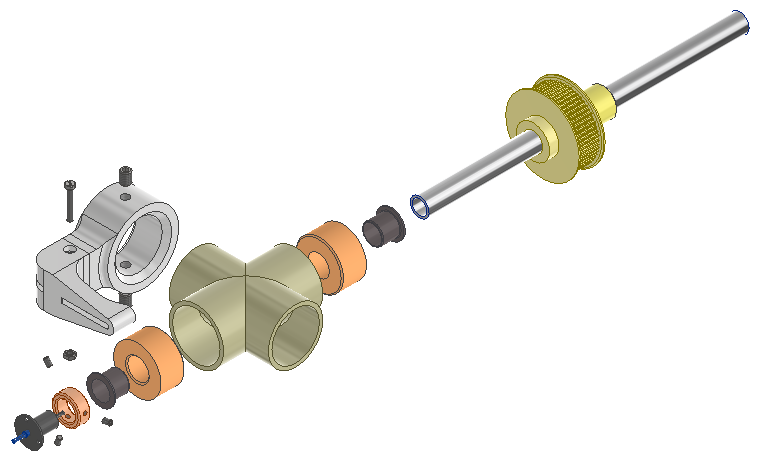
\includegraphics[width=\textwidth]{2_diss}
		\caption{Czwórnik ramy klinostatu.} 
		
		\label{fig:czwórnik}
	\end{subfigure}\vspace{15mm}%
	
	\begin{subfigure}{.8\textwidth}
		\centering
		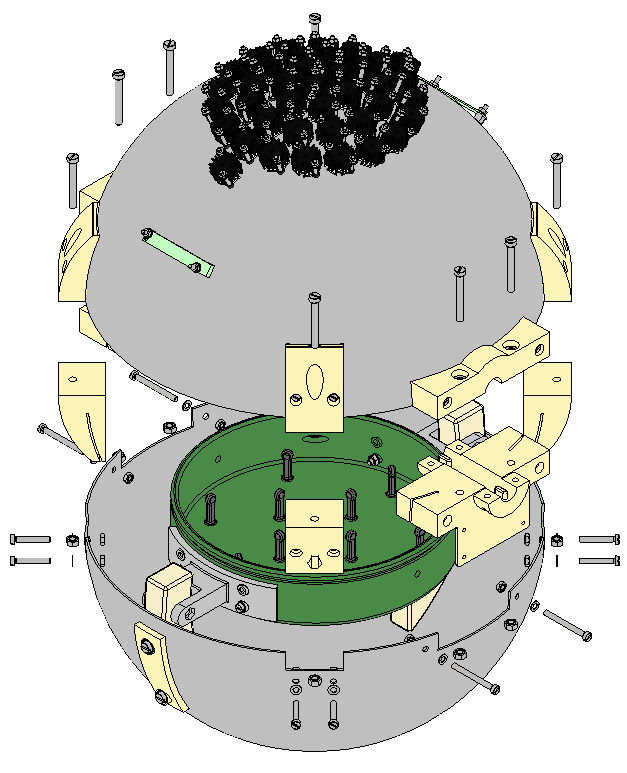
\includegraphics[scale=0.3]{Komora_tweaked_colors_exploded}
		\caption{Komora środowiskowa.} 
		\label{fig:komora}
	\end{subfigure}

	\caption{Przykładowe części modelu komputerowego projektu.}
	\caption*{Źródło: opracowanie własne}
	
\end{figure}


\section{Modyfikacje projektu}

Jako, że projekt rozpoczął się na początku pandemii COVID-19, niemożliwe było prowadzenie prac konstrukcyjnych równolegle z postępem prac modelowych. Spowodowało to zakończenie się projektu na fazie ukończonego modelu komputerowego. Konstrukcję całego urządzenia rozpoczęto rok po zakończeniu się projektu PBL w zespole dwuosobowym w którego skład wchodziłem. Podczas konstrukcji napotkano wiele problemów, które nie zostały przewidziane na etapie prac projektowych i wymagały stworzenia nowych elementów urządzenia, bądź zmodyfikowania już istniejących komponentów. Oprócz tego wymagane było również stworzenie metod konstrukcyjnych tak aby zachować jego kluczowe cechy, oraz aby mogło ono zostać wykonane bez użycia kosztownych metod obróbki takich jak wspomagana numerycznie obróbka maszynowa (ang. \angver{Computerized Numerical Control}, CNC). Takich poprawek stworzono bardzo wiele na drodze konstrukcji urządzenia, natomiast w tym podrozdziale zostaną opisane dwie najbardziej kluczowe dla jego poprawnego działania.


\subsection{Przeciwwaga ramy klinostatu}

Podczas pierwszych prób uruchomieniowych klinostatu napotkano okresowo pojawiający się moment siły, który hamował ruch obrotowy urządzenia przez zbyt duże obciążenie układu napędowego. Za jedno ze źródeł tego problemu zidentyfikowano asymetrię obciążenia ramy klinostatu, powodowaną układem zmiany kierunku pasa układu napędowego komory środowiskowej, który ulokowany jest na rogu ramy. W tym celu na przeciwległym rogu zamontowano przeciwwagę, które generowała moment siły o tym samym kierunku, natomiast o przeciwnym zwrocie. Przeciwwaga składa się z drukowanego uchwytu oraz kawałka rury PP, która wypełniona jest piaskiem w celu zapewnienia odpowiedniej masy. Skonstruowana oraz zamontowana przeciwwaga przedstawiona została na Rys. \ref{fig:przeciwwaga}.

\begin{figure}[ht]
	\centering
	\setlength{\fboxsep}{0pt}
	\setlength{\fboxrule}{1pt}
	\fbox{\includegraphics[scale=0.06]{przeciwwaga}}
	\caption{Zamontowana przeciwwaga.} 
	\caption*{Źródło: opracowanie własne}
	\label{fig:przeciwwaga}
\end{figure}

\subsection{Przekładnie walcowe}

Drugą bardzo istotną dla działania klinostatu modfikacją, był projekt i konstrukcja dwóch przekładni walcowych, które zwiększają dostępny moment obrotowy układu napędowego. Z uwagi na to iż klinostat przeznaczony będzie przedewszystkim do badań nad organizmami roślinnymi, jego prędkość obrotowa powinna mieścić się w zakresie od 1 do 2 RPM. W pierwotnej konfiguracji klinostat był w stanie osiągnąć znacznie większe prędkości obrotowe, co umożliwiło zastosowanie wspomnianych przekładni. Zaprojektowanie przekładnie stosują redukcję obrotów silników 4:1. Pozwala to osiągnąć czterokrotnie wyższy moment obrotowy przed głównym kołem napędowym klinostatu. Model przekładni widoczny jest na Rys. \ref{fig:projekt przekładni}. Przekładnia składa się z dwóch kół zębatych o średnicach kolejno $WSTAWIĆ$ i $WSTAWIĆ$ oraz ilości zębów odpowiednio $WSTAWIĆ$ i $WSTAWIĆ$. Duże koło zębate jest łożyskowane w dwóch miejscach przez konwencjonalne łożyska kulowe, ze względu na to iż przekładnie znajdują się w wystarczająco dużej odległości od objętości jednorodnego pola magnetycznego. Na małym kole zębatym umieszczono dodatkowo wpusty umożliwiajace montaż enkoderów, jeśli zajdzie taka potrzeba. Całość zamknięta została w korpusie odpowiedzialnym za ochronę kół przez pyłem oraz zapobiegającym wydostaniu się smaru na zewnątrz. Skonstruowana przekładna z nałożonym kołem pasowym przedstawiona jest na Rys. \ref{fig:gotowa przekładnia}. Zastosowanie przekładni znacznie poprawiło działanie klinostatu, przy jednoczesnym zachowaniu wymaganej prędkości obrotowej urządzenia.


\begin{figure}
	\centering
	
	\begin{subfigure}[b]{.49\textwidth}
		\centering
		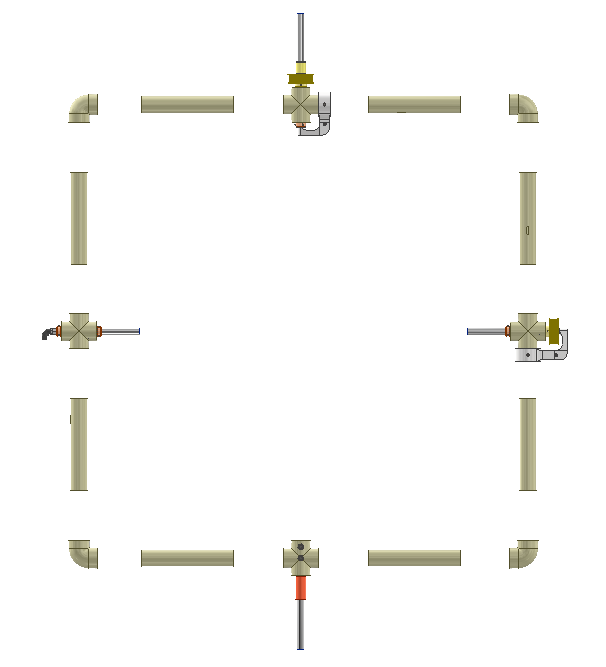
\includegraphics[width=\textwidth]{rama_40_aisass}
		\caption{Projekt przekładni} 
		\label{fig:projekt przekładni}
	\end{subfigure}
	\hfill%
	\begin{subfigure}[b]{.49\textwidth}
		\centering
		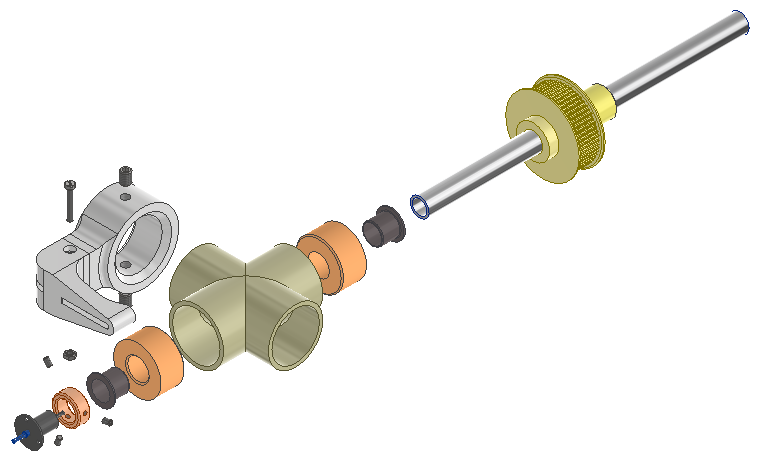
\includegraphics[width=\textwidth]{2_diss}
		\caption{Skonstruowana przekładnia.} 
		
		\label{fig:gotowa przekładnia}
	\end{subfigure}

	\caption{Przekładnie klinostatu.}
	\caption*{Źródło: opracowanie własne}
	
\end{figure}



\section{Napęd klinostatu}

\section{Elektronika układu sterowania}